\section{Definizioni}
\begin{figure}[H]
    \centering
    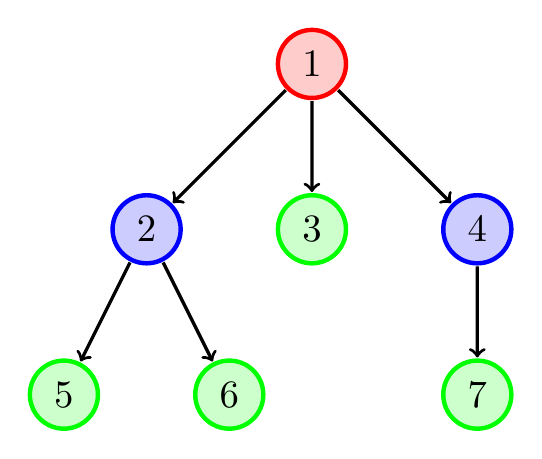
\begin{tikzpicture}[
        scale=1.4, 
        every node/.style={draw=green, fill=green!20, circle, ultra thick, scale=1.4}, 
        edge from parent/.style={draw, very thick}, 
        ->
        ]
    \node[draw=red, fill=red!20]{1}
        child { node[draw=blue, fill=blue!20]{2}
            child { node {5} }
            child { node {6} }
        }
        child { node{3}
        }
        child {node[draw=blue, fill=blue!20] {4} 
            child { node {7} }
        };
    \end{tikzpicture}
    \caption{Esempio albero radicato.}
    \label{fig:example_albero_radicato}
\end{figure}

\begin{itemize}
    \item Un albero radicato per definizione ha \textcolor{red}{\textbf{una sola radice}}, nella \autoref{fig:example_albero_radicato} in questo caso è il \textcolor{red}{nodo 1}.
    \item Un albero radicato ha \textcolor{green}{\textbf{una o più foglie}}, nella \autoref{fig:example_albero_radicato} sono i \textcolor{green}{nodi 3, 5, 6 e 7}.
    \item Un albero radicato può avere \textcolor{blue}{\textbf{uno o più genitori/nodi interni}}, essi per definizione sono nodi che hanno almeno un figlio, cioè che non sono foglie, nella \autoref{fig:example_albero_radicato} sono i \textcolor{blue}{nodi 2, 4} e anche la radice \textcolor{red}{nodo 1} in questo caso è un genitore/nodo interno.
    \item Un albero radicato può essere rappresentato da una coppia di insiemi $T=(V, E)$. Prendiamo come esempio la \autoref{fig:example_albero_radicato}.
    \begin{itemize}
        \item $V$ rappresenta i nodi, detti anche vertici o dall'inglese \emph{\textbf{V}ertexes}. \\
        $V=\{1, 2, 3, 4, 5, 6, 7\}$. 
        \item $E$ rappresenta gli archi, dall'inglese \emph{\textbf{E}dges}. L'insieme è composto a sua volta da coppie di nodi \textit{(genitore, figlio)} dall'insieme $V$. \\
        $E \subset V \times V$\\
        $E=\{(1, 2), (1, 3), (1, 4), (2, 5), (2, 6), (4, 7)\}$. \\
        \textbf{Osservazione}: la radice compare solo a sinistra delle coppie in quanto è l'unico nodo che è solo genitore e non ha genitori. Le foglie invece compaiono solo a destra delle coppie poiché per definizione non hanno figli.
        \item Infine la coppia viene chiamata $T$, dall'inglese \emph{\textbf{T}ree}, cioè albero. \\
        $T=(\{1, 2, 3, 4, 5, 6, 7\},\{(1, 2), (1, 3), (1, 4), (2, 5), (2, 6), (4, 7)\})$. \\
    \end{itemize}
\end{itemize}

\section{Definizione ricorsiva}
\textbf{Passo base}: $T=(\{r\}, \{\emptyset\})$ è un albero radicato

\begin{figure}[H]
    \centering
    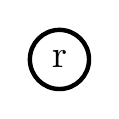
\begin{tikzpicture}[
        scale=1.4, 
        every node/.style={draw, circle, ultra thick, scale=1.4}
        ]
    \node{r};
    \end{tikzpicture}
    \caption{Passo base definizione ricorsiva albero radicato.}
    \label{fig:pb_def_ric_albero_radicato}
\end{figure}

\textbf{Passo ricorsivo}: Supponiamo che $T_1=(V_1, E_1), ..., T_n=(V_n, E_n)$ siano alberi radicati disgiunti, cioè $\displaystyle\bigcap^n_{i=1} V_i = \emptyset$ (gli alberi non hanno nodi in comune). Le respettive radici sono $r_1 \in V_1, ..., r_n \in V_n$.
Allora $T=(V, E)$ si ottiene ponendo come radice un nodo $r \not\in V_1 \cup ... \cup V_n$ e da $r$ si aggiunge un arco a ogni $r_1 \in V_1, ..., r_n \in V_n$. 

$V = \{r\} \cup V_1 \cup ... \cup V_n$

$E = \{(r, r_1), ..., (r, r_n)\} \cup E_1 \cup ... \cup E_n$ \\
$T = (V, E)$ è un albero radicato.

\begin{figure}[H]
    \centering
    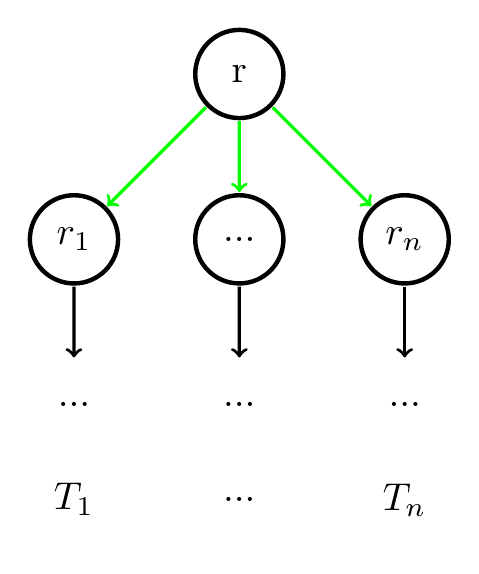
\begin{tikzpicture}[
        scale=1.4, 
        every node/.style={draw, circle, ultra thick, scale=1.4, minimum size=0.8cm},
        edge from parent/.style={draw, very thick},
        norm/.style={draw=black},
        green_edge/.style={draw=green},
        ->
        ]
    \node{r}
        child[green_edge] { node[norm]{$r_1$}
            child[norm] { node[draw=none, label={270:$T_1$}]{...} }
        }
        child[green_edge] { node[norm]{...}
            child[norm] { node[draw=none, label={270:...}]{...} }
        }
        child[green_edge] { node[norm]{$r_n$}
            child[norm] { node[draw=none, label={270:$T_n$}]{...} }
        };
    \end{tikzpicture}
    \caption{Passo ricorsivo definizione ricorsiva albero radicato.}
    \label{fig:pr_def_ric_albero_radicato}
\end{figure}

\section{Numero di vertici}
\textbf{Passo base}: Se $T=(\{r\}, \emptyset)$, allora $|V|=1$

\textbf{Passo ricorsivo}: Se $T=(V, E)$ è un albero radicato costruito a partire dagli alberi $T_1=(V_1, E_1), ..., T_n=(V_n, E_n)$, allora $|V| = 1 + |V_1| + ... |V_n|$. \\
\textbf{N.B.}: L'$1$ rappresenta la radice $r \not\in V_1 \cup ... \cup V_n$, così come definito nel Passo ricorsivo della costruzione dell'albero radicato. Nella \autoref{fig:pr_def_ric_albero_radicato} è il vertice $r$.

\section{Numero di edges(archi)}
\textbf{Passo base}: Se $T=(\{r\}, \{\emptyset\})$, allora $|E| = 0$

\textbf{Passo ricorsivo}: Se $T=(V, E)$ è un albero radicato costruito a partire da $T_1=(V_1, E_1), ..., T_n=(V_n, E_n)$, allora $|E| = n + |E_1| + ... + |E_n|$. \\
\textbf{N.B.}: $n$ sono gli archi dalla radice ai vertici $r_1 \in V_1, ..., r_n \in V_n$, nella \autoref{fig:pr_def_ric_albero_radicato} sono gli archi in verde.

\section{Numero di foglie}
\label{sec:albero_radicato_num_foglie}
Sia $f(T)$ la funzione che prende in input un albero e restituisce il numero di foglie di esso.

\textbf{Passo base}: Se $T=(\{r\}, \emptyset)$, allora $f(T) = 1$

\textbf{Passo ricorsivo}: Se $T=(V, E)$ è un albero radicato costruito a partire da $T_1=(V_1, E_1), ..., T_n=(V_n, E_n)$, allora $f(T) = f(T_1) + ... + f(T_n)$. \\
\textbf{N.B.}: La radice non viene aggiunta al conteggio del numero di foglie, perché $T_1, ..., T_n$ essendo alberi radicati, dal Passo base della definizione di albero radicato sappiamo che hanno almeno un vertice, ossia la radice. Poiché $T$ è costruito a partire da $T_1=(V_1, E_1), ..., T_n=(V_n, E_n)$, la radice di $T$ avrà $n$ figli e per definizione di foglia, non può essere una foglia se ha figli. 

\section{Numero di nodi interni}
Sia $i(T)$ la funzione che prende in input un albero e restituisce il numero di nodi interno di esso.

\textbf{Passo base}: Se $T=(\{r\}, \emptyset)$, allora $i(T) = 0$

\textbf{Passo ricorsivo}: Se $T(V, E)$ è un albero radicato costruito a partire da $T_1=(V_1, E_1), ..., T_n=(V_n, E_n)$, allora $i(T) = 1 + i(T_1) + ... + i(T_n)$. \\
\textbf{N.B.}: L'$1$ è la radice, in quanto nel Passo ricorsivo non è più una foglia. Il perché è spiegato nel "N.B." di \nameref{sec:albero_radicato_num_foglie}.

\section{Altezza di un vertice}
\textbf{N.B.}: L'altezza di un vertice si conta dal basso verso l'alto.
\begin{itemize}
    \item Se $v$ è una foglia, allora l'altezza di $v$ è $0$.
    \item Altrimenti l'altezza di $v$ è la massima altezza tra i figli di $v$ più $1$.
\end{itemize}

\textbf{Osservazione}: L'altezza di un albero è l'altezza della sua radice.

Prendendo come esempio \autoref{fig:example_albero_radicato}, i nodi di colore rosso hanno \textcolor{red}{altezza 2}, quelli di colore blu hanno \textcolor{blue}{altezza 1} e quelli di colore verde hanno \textcolor{green}{altezza 0}.

\section{Profondità di un vertice}
\textbf{N.B.}: La profondità di un vertice si conta dall'alto verso il basso.
\begin{itemize}
    \item Se $v$ è la radice, allora la profondità di v è 0.
    \item Altrimenti la profondità di $v$ è la profondità del padre di $v$ più 1.
\end{itemize}

\begin{figure}[H]
    \centering
    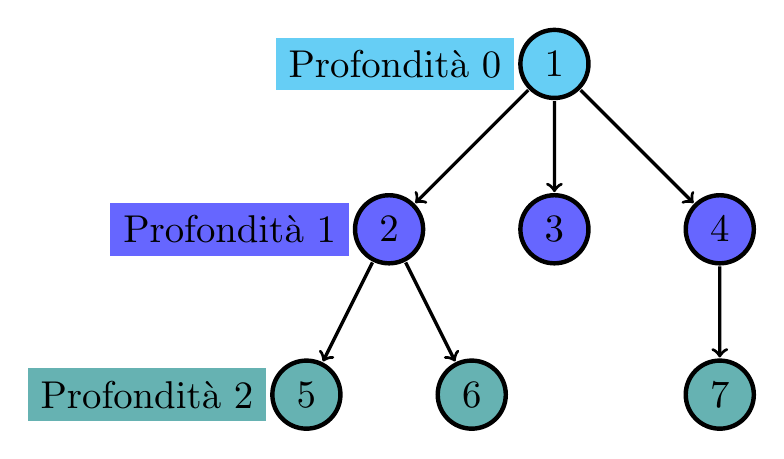
\begin{tikzpicture}[
        scale=1.4, 
        every node/.style={draw, circle, ultra thick, scale=1.4}, 
        edge from parent/.style={draw, very thick},
        label_altezza/.style={rectangle},
        node_prof2/.style={fill=teal!60},
        node_prof1/.style={fill=blue!60},
        ->
        ]
    \node[fill=cyan!60, label={[label_altezza, fill=cyan!60]180:Profondità 0}]{1}
        child { node[node_prof1, label={[label_altezza, node_prof1]180:Profondità 1}]{2}
            child { node[node_prof2, label={[label_altezza, node_prof2]180:Profondità 2}] {5} }
            child { node[node_prof2] {6} }
        }
        child { node[node_prof1]{3}
        }
        child {node[node_prof1] {4} 
            child { node[node_prof2] {7} }
        };
    \end{tikzpicture}
    \caption{Esempio profondità di un vertice.}
    \label{fig:example_profondita_vertice}
\end{figure}

